\documentclass[a4paper, 11pt]{article}
\usepackage{amsmath}
\usepackage{graphicx}

\begin{document}

For a race with a duration of $t$ milliseconds, when we hold down the button for $p$ milliseconds, the distance the boat travels before time runs out is:

\begin{equation*}
    d = (t - p) * p
\end{equation*}

If a record of $r$ milliseconds has been set, how long did that person hold down the button for?
\begin{align*}
    r &= (t - p_r) * p &&\text{solve for $p_r$} \\
    0 &= (t - p_r) * p_r - r \\
    0 &= tp_r - p_r^2 - r \\
    0 &= p_r^2 - tp_r + r &&\text{2nd order polynomial} \\
    p_r &= \frac{1}{2} (t - \sqrt{t^2 - 4r})
\end{align*}

What is the optimal duration to press the button $p_o$? Let's take a look at a scenario where the time of the race is 10 milliseconds:

\begin{figure}[h!]
    \centering
    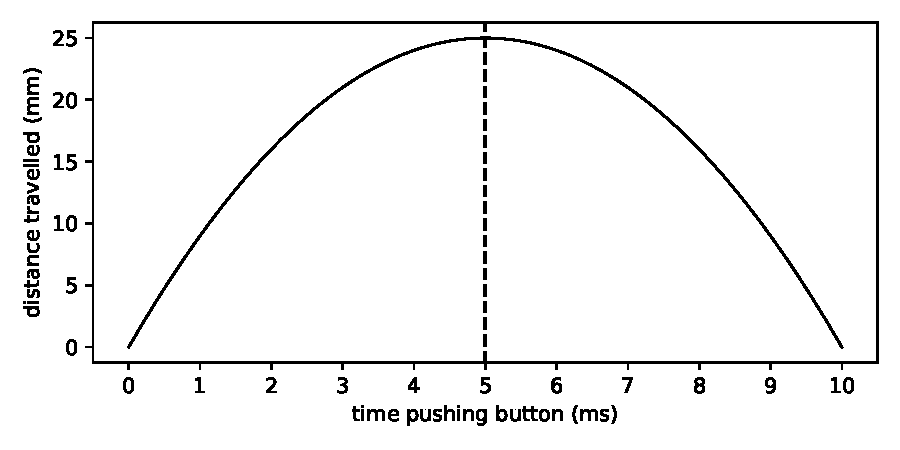
\includegraphics[width=8cm]{fig1.pdf}
\end{figure}

The distance travelled is symmetric.
Hence, the range of button durations that will beat the record is:

\begin{equation*}
    p_r \ldots (t - p_r)
\end{equation*}

Computing the number of integer values in that range $n$:

\begin{equation*}
    n = \lfloor (t - p_r) \rfloor - \lceil p_r \rceil + 1
\end{equation*}

\end{document}
